\chapter{Error propagation}
\label{ch:error-propagation}

All the methods and equations presented thus far have assumed that all
parameters are either known or measured with infinite precision. In
reality, however, the analytical equipment used to measure isotopic
compositions, elemental concentrations and radioactive half-lives is
not perfect.  It is crucially important that we quantify the resulting
analytical uncertainty before we can reliably interpret the resulting
ages.\\

For example, suppose that the extinction of the dinosaurs has been
dated at 65 Ma in one field location, and a meteorite impact has been
dated at 64 Ma elsewhere.  These two numbers are effectively
meaningless in the absence of an estimate of precision. Taken at face
value, the dates imply that the meteorite impact took place 1 million
years after the mass extinction, which rules out a causal relationship
between the two events. If, however, the analytical uncertainty is
significantly greater than 1 Myr (e.g. 64 $\pm$ 2 Ma and 65 $\pm$ 2
Ma), then such of a causal relationship remains very plausible.

\section{Some basic definitions}
\label{sec:summarystatistics}

Suppose that our geochronological age ($t$) is calculated as a function
($f$) of some measurements ($x$ and $y$):

\begin{equation}
t = f(x,y)
\label{eq:tfxy}
\end{equation}

Suppose that we have performed a large number ($n$) of replicate
measurements of $x$ and $y$:

\begin{equation}
\left\{
\begin{array}{rl}
x = & \{x_1, x_2, \cdots, x_i, \cdots, x_n\} \\
y = & \{y_1, y_2, \cdots, y_i, \cdots, y_n\}
\end{array}
\right.
\label{eq:xy}
\end{equation}

It is useful to define the following \emph{summary statistics}:

\begin{enumerate}
\item The mean:
\begin{equation}
\left\{
\begin{array}{rl}
\overline{x} \equiv & \frac{1}{n} \sum_{i=1}^{n} x_i\\
\overline{y} \equiv & \frac{1}{n} \sum_{i=1}^{n} y_i
\end{array}
\right.
\label{eq:mean}
\end{equation}

is a useful definition for the `most representative' value of $x$ and
$y$, which can be plugged into Equation~\ref{eq:tfxy} to calculate the
`most representative' age.

\item The variance:
\begin{equation}
\left\{
\begin{array}{rl}
s[x]^2 \equiv & \frac{1}{n-1} \sum_{i=1}^{n} (x_i-\overline{x})^2\\
s[y]^2 \equiv & \frac{1}{n-1} \sum_{i=1}^{n} (y_i-\overline{y})^2
\end{array}
\right.
\label{eq:variance}
\end{equation}

with $s[x]$ and $s[y]$ the `standard deviations', is used to quantify
the amount of dispersion around the mean.

\item The covariance:
\begin{equation}
s[x,y] \equiv \frac{1}{n-1} \sum_{i=1}^{n} (x_i-\overline{x})(y_i-\overline{y})
\label{eq:covariance}
\end{equation}

quantifies the degree of correlation between variables $x$ and $y$.
\end{enumerate}

$\overline{x}$, $\overline{y}$, $s[x]^2$, $s[y]^2$ and $s[x,y]$ can
all be estimated from the input data $(x,y)$. These values can then be
used to infer $s[t]^2$, the variance of the calculated age $t$, a
process that is known as `error propagation'. To this end, recall the
definition of the variance (Equation \ref{eq:variance}):

\begin{equation}
s[t]^2 \equiv \frac{1}{n-1} \sum_{i=1}^{n} (t_i-\overline{t})^2
\label{eq:vart}
\end{equation}

We can estimate $(t_i-\overline{t})$ by differentiating Equation
\ref{eq:tfxy}:

\begin{equation}
t_i - \overline{t} = (x_i-\overline{x}) \frac{\partial f}{\partial x} +
(y_i-\overline{y}) \frac{\partial f}{\partial y}
\label{eq:ti-t}
\end{equation}

Plugging Equation \ref{eq:ti-t} into \ref{eq:vart}, we obtain:

\begin{align}
s[t]^2 & = \frac{1}{n-1} \sum_{i=1}^{n} \left[
(x_i-\overline{x}) \left(\frac{\partial f}{\partial x}\right) +
(y_i-\overline{y}) \left(\frac{\partial f}{\partial y}\right) \right]^2 \label{eq:s2t1}\\
~ & = s[x]^2 \left(\frac{\partial f}{\partial x}\right)^2 +
s[y]^2 \left(\frac{\partial f}{\partial y}\right)^2 +
2~s[x,y] \frac{\partial f}{\partial x} \frac{\partial f}{\partial y} \label{eq:s2t}
\end{align}

This is the general equation for the propagation of uncertainty with
two variables, which is most easily extended to more than two
variables by reformulating Equation \ref{eq:s2t} into a matrix form:

\begin{equation}
s[t]^2 = 
\left[
\begin{array}{@{}c@{~}c@{}}
\frac{\partial t}{\partial x}&\frac{\partial t}{\partial y}
\end{array}
\right]
\left[
\begin{array}{@{}c@{~}c@{}}
s[x]^2 & s[x,y]\\
s[x,y] & s[y]^2
\end{array}
\right]
\left[
\begin{array}{@{}c@{}}
\frac{\partial t}{\partial x} \\
\frac{\partial t}{\partial y}
\end{array}
\right]
\label{eq:s2tmatrix}
\end{equation}

where the innermost matrix is known as the \emph{variance-covariance}
matrix and the outermost matrix (and its transpose) as the
\emph{Jacobian matrix}.  Let us now apply this equation to some simple
functions.

\section{Examples}

Let $x$ and $y$ indicate measured quantities associated with
analytical uncertainty.  And let $a$ and $b$ be some error free
parameters.

\begin{enumerate}
\item{addition:}
\begin{align}
& t = a x + b y \Rightarrow \frac{\partial t}{\partial x} = a, 
\frac{\partial t}{\partial y} = b \nonumber\\
& \Rightarrow s[t]^2 = a^2 s[x]^2 + b^2 s[y]^2 + 2ab~s[x,y]
\label{eq:addition}
\end{align}

\item{subtraction:}
\begin{equation}
t = a x - b y \Rightarrow
s[t]^2 = a^2 s[y]^2 + b^2 s[y]^2 - 2ab~s[x,y]
\label{eq:subtraction}
\end{equation}

\item{multiplication:}
\begin{align}
& t = a x y \Rightarrow \frac{\partial t}{\partial x} = a y, 
\frac{\partial t}{\partial y} = ax \nonumber\\
& \Rightarrow s[t]^2 = (ay)^2 s[x]^2 + (ax)^2 s[y]^2 + 2a^2 xy~s[x,y] \nonumber\\
& \Rightarrow \left(\frac{s[t]}{t}\right)^2 = \left(\frac{s[x]}{x}\right)^2 + 
  \left(\frac{s[y]}{y}\right)^2 + 2 \frac{s[x,y]}{x y}
\label{eq:multiplication}
\end{align}

\item{division:}
\begin{equation}
t = a \frac{x}{y} \Rightarrow
\left(\frac{s[t]}{t}\right)^2 = \left(\frac{s[x]}{x}\right)^2 + 
  \left(\frac{s[y]}{y}\right)^2 - 2 \frac{s[x,y]}{x y}
\label{eq:division}
\end{equation}

\item{exponentiation:}
\begin{equation}
t = a~e^{bx} \Rightarrow \frac{\partial f}{\partial x} = ab~e^{bx} 
\Rightarrow s[t]^2 = (b t)^2 s[x]^2
\label{eq:exponentiation}
\end{equation}

\item{logarithms:}
\begin{equation}
t = a~\ln(bx) \Rightarrow \frac{\partial f}{\partial x} = \frac{a}{x}
\Rightarrow s[t]^2 = a^2 \left(\frac{s[x]}{x}\right)^2
\label{eq:logarithms}
\end{equation}

\item{power:}
\begin{equation}
  t = a x^b \Rightarrow \frac{\partial f}{\partial x} = b \frac{a
    x^b}{x} \Rightarrow \left(\frac{s[t]}{t}\right)^2 =
  b^2\left(\frac{s[x]}{x}\right)^2
\label{eq:power}
\end{equation}

\end{enumerate}

\section{Accuracy vs. precision}

Recall the definition of the arithmetic mean (Equation \ref{eq:mean}):

$$\overline{x} \equiv \frac{1}{n} \sum_{i=1}^{n} x_i$$

Applying the equation for the error propagation of a sum (Equation
\ref{eq:addition}):

\begin{equation}
s[\overline{x}]^2 = \frac{1}{n} \sum_{i=1}^{n} s[x_i]^2 =
\frac{s[x]^2}{n}
\label{eq:varianceofthemean}
\end{equation}

where we assume that all $n$ measurements were done
\emph{independently}, so that $cov(x_i,x_j)=0 \forall i, j$.  The
standard deviation of the mean is known as the \underline{standard
  error}:

\begin{equation}
s[\overline{x}] = \frac{s[x]}{\sqrt{n}}
\label{eq:standarderror}
\end{equation}

This means that the standard error of the mean monotonically decreases
with the square root of sample size. In other words, we can
arbitrarily increase the \emph{precision} of our analytical data by
acquiring more data. However, it is important to note that the same is
generally not the case for the \emph{accuracy} of those data. The
difference between precision and accuracy is best explained by a darts
board analogy:\\

\noindent
\begin{minipage}{\textwidth}
  \centering
  \ifpdf
  \def\svgwidth{\textwidth}
  \input{bullseye.pdf_tex}
  \else
  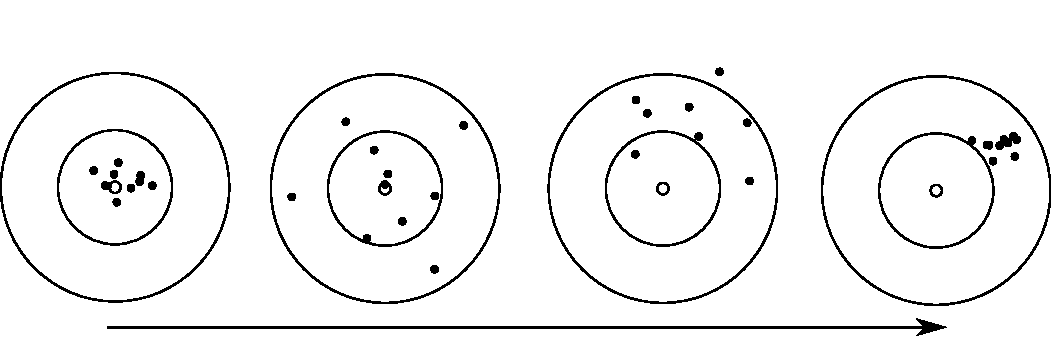
\includegraphics[width=10cm]{../figures/bullseye.png}
  \fi
\end{minipage}

\bigskip

Whereas the analytical precision can be computed from the data using
the error propagation formulas introduced above, the only way to get a
grip on the accuracy is by analysing another sample of independently
determined age. Such test samples are also known as `secondary
standards'.

\ifpdf
\ifuclnotes
\begin{figure}[!ht]
  \centering
  \def\svgwidth{\textwidth}
  \input{covariance.pdf_tex}
  \caption{Four datasets of 100 random numbers (black dots) which have
    the same means (white squares) but different (co-)variance
    structures. The marginal distributions of the $x$ and $y$ variables
    are shown as `bell curves' on the top and right axis of each
    plot.}
  \label{fig:covariance}
\end{figure}
\else % end of uclnotes
\begin{figure}[!ht]
  \noindent\begin{minipage}[t]{.7\textwidth}
\strut\vspace*{-\baselineskip}\newline
\def\svgwidth{\textwidth}
\input{covariance.pdf_tex}
\end{minipage}
\begin{minipage}[t]{.3\textwidth}
  \captionof{figure}{Four datasets of 100 random numbers (black dots) which have
    the same means (white squares) but different (co-)variance
    structures. The marginal distributions of the $x$ and $y$ variables
    are shown as `bell curves' on the top and right axis of each
    plot.}
  \label{fig:covariance}
\end{minipage}
\end{figure}
\fi % end of pdf
\else
\includegraphics[width=10cm]{../figures/covariance.png}
  \captionof{figure}{Four datasets of 100 random numbers (black dots) which have
    the same means (white squares) but different (co-)variance
    structures. The marginal distributions of the $x$ and $y$ variables
    are shown as `bell curves' on the top and right axis of each
    plot.}
  \label{fig:covariance}
\fi
